\section{Simulation}
\label{sec:simulation}

\subsection{Design}
\label{sec:sim-design}

The samples are drawn from model \eqref{eq:model} with $X_1 \equiv 1$, the
other linear covariates independent and standard normal, the modulators
independent of $\bX$, independent of each other and uniform on $[0,1]$, and
Gaussian errors. The levels are $(\lvl{1},\lvl{2},\lvl{3},\lvl{4}) =
(1, 2, -1.5, 0.5)$, repeated cyclically when $p > 4$, and each nonzero
component is a test function centered and scaled to have unit norm in
$L_2[0,1]$. Unless it is fixed, the standard deviation of the error is that of
the regression function over the sample divided by a signal to noise ratio.

The core design has five cells. In the smooth cell, with $(p,q) = (3,2)$, the
first coefficient is additive in the two modulators, with $\gcomp{1}{1}$ and
$\gcomp{1}{2}$ proportional to $\sin(2\pi u)$ and to the cubic
$u^{3} - 1.4u^{2} + 0.4u$, the second varies with $U_1$, with $\gcomp{2}{1}$
proportional to $\cos(4\pi u)$, the other components are zero, and the signal
to noise ratio is 4. The uneven cell keeps this structure, the cosine and the
ratio, and replaces the sine by a Gaussian bump of standard deviation $0.10$
at $0.40$ minus $0.8$ times one of standard deviation $0.018$ at $0.72$, and
the cubic by the chirp $\sin\{2\pi(u + 3.5u^{2})\}$, whose frequency goes from
one to eight cycles over the interval; both are multiplied by an infinitely
differentiable window that equals one on $[0.08, 0.92]$ and vanishes with all
its derivatives at $0$ and $1$ (Section~S9 of the Supplementary Material).
These components are infinitely differentiable, within the smoothness
conditions of the spline theory of \citet{Xue-Yang-2006}, but the scale of two
of them changes along the interval. The inhomogeneous cell keeps the
structure, with the bumps, blocks and heavisine functions of
\citet{Donoho-Johnstone-1994} in place of the sine, the cubic and the cosine,
and signal to noise ratio 3. The mixed cell places the components of the
inhomogeneous one in a model with $(p,q) = (4,4)$, so that 3 of its 16 blocks
are active, with the same ratio. In the null cell every component is zero and
the model is a linear regression with $(p,q) = (3,2)$; the standard deviation
of the error is fixed at $0.62$, about a quarter of that of the regression
function.

In the terms of Assumption~\ref{ass:besov}, the effective regularity is
$\seff = 3/2$ in the smooth cell, where the cubic has different slopes at the
two ends of the interval and its periodic extension has a corner, and
$\seff = 1/2$ in the inhomogeneous and mixed cells, where blocks and heavisine
jump inside the interval. The components of the uneven cell have infinitely
differentiable periodic extensions, and their regularity is limited only by
the vanishing moments of the wavelet.

Each cell is run at $n = 250$, $500$, $1000$ and $2000$, with 100 replicates
of each pair of cell and sample size. A replicate consists of a training
sample of size $n$, a test sample of size 2000 from the same law, with errors
at the standard deviation of the training sample, and a partition of the
training sample into 10 folds; the three are shared by every method, so that
the comparisons within a replicate are paired.

Three arms change one factor at a time in the inhomogeneous and the mixed
cells, at $n = 1000$ and with 100 replicates each. In the first, the signal to
noise ratio is 1 instead of 3. In the second, the modulators are coupled by a
Gaussian copula with correlation $0.5$ between every pair, which keeps the
uniform marginals and makes the cross terms of the Gram matrix between
distinct modulators nonzero; the density of this copula is unbounded at two
corners of the unit square and vanishes at the other two, so that this arm
lies outside Assumption~\ref{ass:U}. In the third arm the linear covariates
depend on the modulating ones: each non-constant covariate is drawn as
$X_\cv = (1-\rho^2)^{1/2} \zeta_\cv + \rho\, h(U_{\cv-1})$ with $\rho = 0.5$,
where $\zeta_\cv$ is standard normal and $h(u) = \sqrt{12}\,(u - 1/2)$ is the
standard score of a uniform modulating covariate, so that $X_2$ is paired with
$U_1$, the modulating covariate of its own coefficient. Each $X_\cv$ keeps
unit variance and has correlation $\rho$ with its pair, and given $\bU$ the
non-constant covariates have covariance $(1-\rho^2)I$, so that the eigenvalue
condition of Assumption~\ref{ass:X} holds while the Gram matrix of the
products no longer factorizes as a Kronecker product. Gaussian covariates are
not bounded, in this arm as in every cell, so that the design lies outside the
bound $B_X$ of Assumption~\ref{ass:X}; what the third arm exercises is the
eigenvalue condition, the part of that assumption that allows the covariates
to depend on the modulators. A replicate of an arm is drawn from the seeds of
the same replicate of its core cell, and the first and the third arms share
with it the modulators, the draws $\zeta_\cv$ and the standardized errors.

A larger model has $(p,q) = (6,4)$ at $n = 1000$, with 24 blocks of which
6 are active: the active structure of the inhomogeneous cell twice, on
$(X_1,X_2)\times(U_1,U_2)$ and on $(X_3,X_4)\times(U_3,U_4)$, with $\beta_5$
and $\beta_6$ constant and signal to noise ratio 3.

Every sample is derived from a single master seed, through an injective
encoding of the cell, the sample size, the replicate and the stream. The seeds
are independent of those of the pilot runs on which the estimator, its tuning
rules and the grids below up to $n = 1000$ were settled, so that the study does not evaluate
the method on the samples on which it was chosen.

\subsection{Methods and tuning}
\label{sec:sim-methods}

Every method is tuned in its own terms, by the criteria it is used with, so
that a difference between two methods is not a difference of tuning. The WAFC
is the estimator \eqref{eq:estimator} with $b = \lceil\log n\rceil$ and
weights $|G|^{1/2}$, on the periodized extremal phase wavelets of
\citet{Daubechies-1992} with four vanishing moments ($L = 8$), evaluated by
table and with no margin; $(J,\pen)$ is chosen by 10-fold cross-validation
(Section~\ref{sec:tuning}) and the threshold by the one standard error rule on
the same folds (Section~\ref{sec:threshold}), the default of the software. The
row WAFC (cv) comes from the same search, with the threshold that minimizes
the cross-validated error, the option aimed at prediction. Seven other rows
enter the tables, five competitors and two references.

GAM (REML) and GAM (GCV) fit the additive varying coefficient model by
penalized regression splines with the \texttt{mgcv} package
\citep{Wood-2017,Wood-mgcv-2025}, through its function \texttt{bam}
\citep{Wood-Goude-Shaw-2015}, with one smooth of $U_\md$ multiplied by $X_\cv$
for every block and an extra penalty on the null space of each smooth, which
lets a smooth be shrunk to zero \citep{Marra-Wood-2011}. The first chooses the
smoothing parameters by restricted maximum likelihood and the second by
generalized cross-validation, and each chooses the basis dimension $k$, common
to the smooths, from a grid by its own criterion, which is the full search of
\citet{Ruppert-2002} and the search of \citet[Section~2.3]{Pya-Wood-2016}. GAM
(GCV) is not run in the mixed cell or in the larger model, where a single fit
at the top of its grid takes more than an hour.

The B-spline group lasso expands each component in cubic B-splines, centered
on the training sample, and fits a group lasso \citep{Yuan-Lin-2006} with one
group per block and the levels unpenalized, with \texttt{grpreg}; the number
of basis functions per block, $2^J$, and the penalty are chosen by
cross-validation on the folds. It differs from the WAFC in the basis and in
the unit of the penalty, a whole block instead of a chunk.

The adaptive spline gives each block a cubic spline with its own knots, chosen
from the data, in the spirit of \citet{Wang-Jiang-Liu-2024}, who choose the
knots by dynamic programming in a model with a single modulator. Here the
knots of a block, at most 12 among 40 candidates at quantiles of its
modulator, are inserted one at a time by the Bayesian information criterion,
inside a backfitting cycle over the blocks, so that this row stands in for
their method and does not implement it.

The block lasso (KP) is the estimator of \citet{Klopp-Pensky-2015} on the
wavelet design of the WAFC, with their chunk size $\lceil\log n\rceil$ and the
levels penalized as one more group, as in their norm. It departs from their
estimator in the chunks, which stay inside a resolution level, each coarse
level being a chunk of its own, and in the weights, which are the $|G|^{1/2}$
of the solver; it differs from the WAFC in the penalized levels and in the
cut of the chunks. Its $(J,\pen)$ is chosen by cross-validation, with no
threshold.

The two references are the oracle support, the estimator
\eqref{eq:estimator} on the columns of the active blocks only, with $(J,\pen)$
chosen by cross-validation and no threshold, whose distance to the WAFC is the
price of not knowing the structure; and the constant coefficients, least
squares on $\bX$ alone, which is the correct model in the null cell, where the
oracle support reduces to it, and a floor in the others. The coordinatewise
lasso of Section~\ref{sec:computation}, at the pair chosen by
cross-validation and thresholded by the one standard error rule, is reported
in Section~S9 of the Supplementary Material.

The grids were fixed by the pilot runs and do not depend on the cell:
$J \in \{2,\dots,8\}$ for the methods on the wavelet design, the same $J$ for
the $2^J$ B-splines per block, and $k \in \{5, 10, 20, 40, 80\}$ for the two
searches of \texttt{mgcv}, one grid for both criteria, which avoids powers of
two so that the splines are not tuned on the grid of the wavelets. A
resolution is capped by the number of distinct points of the modulator: at
$n = 250$ the 255 wavelets of $J = 8$ exceed the 249 distinct points that a
modulator has on the circle after rescaling, where its two extremes meet at
$0 \equiv 1$, so the level is built as $J = 7$ and the effective grid there
is $\{2,\dots,7\}$, and the dimension 256 of the B-splines is dropped. At
$n = 2000$, and only there, the grids are extended before the study, to
$J \in \{2,\dots,9\}$ for the methods on the wavelet design and for the
B-splines, and with $k = 120$ added to the grid of \texttt{mgcv}, because the
resolution that the theory prescribes grows with $n$, as in \eqref{eq:Jn}.
The grid of GAM (REML) is extended further, to $k = 160$ at $n = 1000$ and
$k = 240$ at $n = 2000$, where its choice would otherwise sit at the top of
the grid in the cells with inhomogeneous components; Section~S9 of the
Supplementary Material gives the rules that leave a candidate out.

\subsection{Measures}
\label{sec:sim-measures}

Every method is asked the same questions on the test sample and on a grid of
256 equally spaced points in the observed range of each modulator. The
prediction error is the root mean squared difference between the fitted and
the true regression function on the test sample. The error of the components
is the integrated squared error summed over the blocks, with the fit and the
truth both centered on the grid, because every method fixes the level of a
component by its own convention; it is split between the active blocks and
the null ones, where it measures what a method puts where there is nothing.
The two errors are reported separately, since a method can predict well with
wrong components, or the reverse. The structure is read from the blocks a
method keeps, as the frequency $\Prob(\widehat{\mathcal{S}} = \mathcal{S})$ of
the replicates in which they are exactly the active ones, beside the mean
numbers of null blocks kept and of active blocks dropped; a smooth of
\texttt{mgcv} counts as kept when its effective degrees of freedom exceed
$0.1$, since the extra penalty shrinks it toward zero but never to zero
exactly. The time is the elapsed time of a fit, the search over the grids and
the threshold included, in a single process on one core of an Intel Core
i9-10900KF, ten fits at a time on its ten cores. Means over
the replicates are reported with their standard errors; since the methods
share the samples of a replicate, the Supplementary Material also gives the
median, within replicate, of the ratio of each error to that of the WAFC, and
the fraction of replicates in which a method has the smaller error.

\subsection{Results}
\label{sec:sim-results}

Table~\ref{tab:sim-main} gives the errors and the recovery of the structure at
$n = 1000$, and Figure~\ref{fig:sim-components} the fitted components of the
inhomogeneous cell. The WAFC recovers the structure exactly in every replicate
of every cell, which no competitor does in more than 36\% of the replicates of
any cell: GAM (REML) keeps about one null block per replicate in the cells with
three active blocks and close to five of the 13 null blocks of the mixed cell
(Section~S9 of the Supplementary Material). In the inhomogeneous and the mixed
cells, where the components are spatially inhomogeneous, it is also the most
accurate of the methods that do not know the structure: its error is 9\% and
4\% below that of GAM (REML), and smaller in 95\% and 82\% of the paired
replicates, and within 3\% and 8\% of that of the oracle support, which is the
price of not knowing the structure. In the smooth and the uneven cells, whose
components are infinitely differentiable, the splines are in their own
setting and predict better, GAM (REML) by 20\% and 9\%; there the WAFC stays
within 6\% of the oracle support and keeps the exact structure, which GAM
(REML) finds in 21\% and 36\% of the replicates. In the null cell the
threshold removes every block, and the WAFC coincides with the constant
coefficients, the correct model, while the methods that keep null blocks have
errors from 47\% to 230\% above it. In Figure~\ref{fig:sim-components} the
pointwise median of the WAFC reaches a larger part of the height of each of
the eleven peaks of the bumps, above the baseline, than that of GAM (REML), by
14\% to 44\%, and the two follow the jumps of the blocks, both below the
truth between 0.3 and 0.4 (0.53 and 0.63 against 0.75); the pointwise
quantiles are in Figure~S1 of the Supplementary Material.

Across sample sizes the comparison of prediction depends on $n$. In the
inhomogeneous cell GAM (GCV) is ahead at $n = 250$ and $500$, by 6\% and 5\%,
and behind from $n = 1000$; GAM (REML) is behind at $n = 500$ and $1000$ and
ahead at $n = 2000$, by 2\% in the inhomogeneous cell and 6\% in the mixed
one, with its grid extended to $k = 240$, at 15 times the time of the WAFC in
the mixed cell and without the exact structure in any of its replicates. The
WAFC recovers the structure in 36\% and 25\% of the replicates of these two
cells at $n = 250$, in 91\% and 84\% at $n = 500$, and in every replicate of
the other cells at every $n$. The slopes of the logarithm of the errors
against $\log n$ are close to those of the oracle support in every cell.

In the arms, the copula and the dependent covariates leave the comparison as
in the core cells. With signal to noise ratio 1 the WAFC recovers the
structure in 6\% and 7\% of the replicates: it keeps almost no null block and
drops 1.2 active blocks on average, because the error of a fitted active
component, about 0.77 in $L_2[0,1]$, is then close to the unit norm of the
block, and the window of Corollary~\ref{cor:threshold}(iii) closes; GAM
(REML) and GAM (GCV), which do not threshold, predict better by 4\% and 10\%.
With the threshold of the smallest cross-validated error, which keeps more
blocks, the WAFC recovers the structure in 62\% and 47\% of the replicates
and predicts better than GAM (REML), by 4\% and 3\%.
In the larger model, with 24 blocks of which 6 are active, the WAFC has an
error 3\% below that of GAM (REML) and recovers the structure in 65\% of the
replicates, dropping one active block in the others, while GAM (REML) keeps
6.4 null blocks on average. A fit of the WAFC with its tuning takes 40 to 80
seconds at $n = 1000$, against about 45 for GAM (REML), 430 in the mixed
cell, and 80 to 240 for GAM (GCV). Section~S9 of the Supplementary Material
gives the errors at every sample size, the arms and the larger model,
the structure, the resolution and the dimension chosen with the frequency of
choices at the top of a grid, the time, and the slope of the logarithm of the
errors against $\log n$. [E7: the address of the compendium that reproduces
the study.]

% tables/sim-main_6.tex -- Table 1 do ms_6.tex (E5b, 2026-10-12), o lugar de
% tables/sim-main.tex da k = 5 com os numeros da E4.4. Gerada de
% results/tables/core/summary.csv em n = 1000 (o compendio e a verdade): (a) rmse_f_mean,
% com a faixa de rmse_f_se (0.00122 a 0.00552) na legenda, pela largura; (b) exact_support. O ISE das componentes fica na Table S1 (em espaco
% duplo, as instrucoes da SS, tres paineis passavam da pagina); o painel (b) sem o oraculo
% (1 por construcao) e os coeficientes constantes (0, e 1 na nula). Linhas na ordem de
% config/study.yaml, com os rotulos de la; o VCBART e o lasso coordenado ficam fora do
% corpo (D60(d); o lasso vai a S9). Colunas da celula mais suave a mais dificil, a nula
% por ultimo. O GAM (GCV) nao roda na mixed. \color{colR1} dentro do float (D75(d)).
\begin{table}[tp]
\caption{Simulation at $n = 1000$, 100 replicates per cell: (a) root mean
squared error of prediction (standard errors 0.001 to 0.006); (b) frequency
of the exact structure. GAM (GCV) is not run in the mixed cell.}
\label{tab:sim-main}
\centering
\small
\begin{tabular}{lccccc}
\hline
 & Smooth & Uneven & Inhomogeneous & Mixed & Null \\
\hline
\multicolumn{6}{l}{(a) Prediction error} \\
WAFC & 0.165 & 0.247 & 0.768 & 0.820 & 0.030 \\
WAFC (cv) & 0.169 & 0.251 & 0.771 & 0.822 & 0.044 \\
GAM (REML) & 0.131 & 0.224 & 0.836 & 0.854 & 0.048 \\
GAM (GCV) & 0.144 & 0.222 & 0.785 & -- & 0.070 \\
B-spline group lasso & 0.208 & 0.308 & 0.941 & 0.975 & 0.045 \\
Adaptive spline & 0.159 & 0.250 & 1.047 & 1.085 & 0.100 \\
Block lasso (KP) & 0.175 & 0.263 & 0.796 & 1.015 & 0.065 \\
Oracle support & 0.157 & 0.234 & 0.748 & 0.758 & 0.030 \\
Constant coefficients & 1.733 & 1.738 & 1.738 & 1.727 & 0.030 \\
\hline
\multicolumn{6}{l}{(b) Frequency of the exact structure, $\Prob(\widehat{\mathcal{S}} = \mathcal{S})$} \\
WAFC & 1.00 & 1.00 & 1.00 & 1.00 & 1.00 \\
WAFC (cv) & 0.71 & 0.72 & 0.88 & 0.84 & 0.21 \\
GAM (REML) & 0.21 & 0.36 & 0.28 & 0.02 & 0.07 \\
GAM (GCV) & 0.11 & 0.09 & 0.09 & -- & 0.03 \\
B-spline group lasso & 0.00 & 0.00 & 0.00 & 0.00 & 0.19 \\
Adaptive spline & 0.00 & 0.00 & 0.00 & 0.00 & 0.00 \\
Block lasso (KP) & 0.00 & 0.00 & 0.00 & 0.00 & 0.05 \\
\hline
\end{tabular}
\end{table}

% figures/sim-components_6.tex -- Figure 1 do ms_6.tex (E5b, 2026-10-12), o lugar de
% figures/sim-components.tex da k = 5. A figura e figures/sim-components.pdf, gerada por
% figures/make-sim-components.R dos curves.csv da E4.4 (so na desktop; SHA-256 no
% results/README.md): as medianas ponto a ponto das 100 replicas, numa grade comum. A
% opcao com as faixas vai ao supp (Figure S1), a da replica de ISE mediano foi descartada
% (escolha do autor, E5b). Legivel em preto e branco, sem cor na legenda (SS).
% \color{colR1} dentro do float (D75(d)).
\begin{figure}[t]
\centering
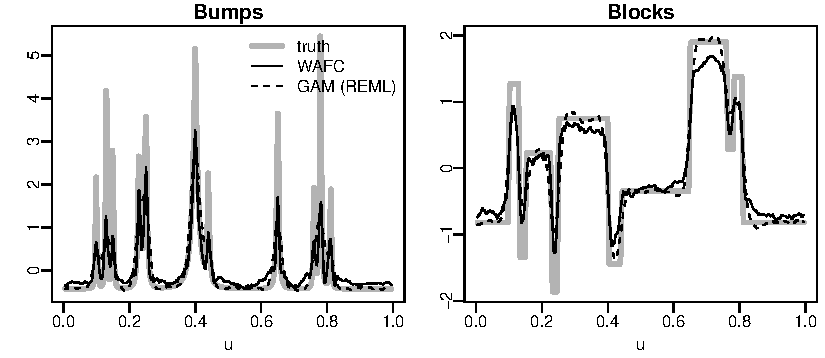
\includegraphics[width=\textwidth]{figures/sim-components.pdf}
\caption{Inhomogeneous cell, $n = 1000$: the components $\gcomp{1}{1}$
(bumps, left) and $\gcomp{1}{2}$ (blocks, right). The thick line is the
truth, and the solid and dashed lines are the pointwise medians over the 100
replicates of the WAFC and of GAM (REML); Figure~S1 of the Supplementary
Material adds the pointwise 5\% and 95\% quantiles.}
\label{fig:sim-components}
\end{figure}



%%%%%%%%%%%%%%%%%%%%%%%%%%%%%%%%%%%%%%%%%%%%%%%%%%%%%%%%%%%%%%%%%%%%%%%%%%%%%%
% E5h (k = 5): a Secao 6 sem os numeros. Os dados, o modelo e as leituras sao os
% de D56, D57, D59, D64, D66 e D67, como o compendio os executa
% (wafc-studies/config/application.yaml, R/application_data.R, R/application.R,
% R/application_report.R, data/README.md); as fontes sao as de L12 e L13. Os
% numeros ficam como [E6.2: ...], a trocar pelos de readings-, prediction- e
% structure-marylebone.ukair.csv da rodada. E5j (2026-10-07): os de marylebone
% trocados pelos de results/tables/ (handoff-E5j.md, cada numero e a sua
% coluna); a frase dos buracos no 6.1 (D73, "spacing" no lugar de "support"),
% o pico na segunda metade de 2003 e a serie de Carslaw ate dezembro de 2003
% (respostas do autor na E5j). Os da beijing.heat (6.4) ficam. E5k (2026-10-08): o
% do 6.4 trocado pelo de prediction-beijing.heat.csv (ratio_best_spline e wins do
% wafc.cv1se); no 6.3, D76(b) com os numeros que o drawn_grid() da E6.2b mudou
% (rise 9.0, 9.4 a 10.3; fraction_at_2003-01-01 0.17 a 0.36; date_90 em 18 das 20
% particoes antes do buraco de 2003, nas outras duas e no gam.reml no primeiro ponto
% desenhado depois dele; peak_above_before 13.5) e a oracao de D76(c). A frase de Opsomer, Wang e Yang (2001)
% nao entra (D65). As atribuicoes que as licencas pedem estao nos
% Acknowledgements.

